\section{Éclairage à l'aide de la méthode de Phong}

Pour gérer l'éclairage nous utilisons la méthode de Phong, qui divise les lumières en trois catégories~:
\begin{itemize}
    \item composante ambiante
    \item composante diffuse (gestion de la diffusion de la lumière au sein d'une face)
    \item composante spéculaire (gestion des reflets).
\end{itemize}

Au sein de ce système, nous avons implémenté trois différents types de lumières~:
\begin{itemize}
    \item lumière directionnelle
    \item lumière localisée
    \item projecteur.
\end{itemize}

{\centering 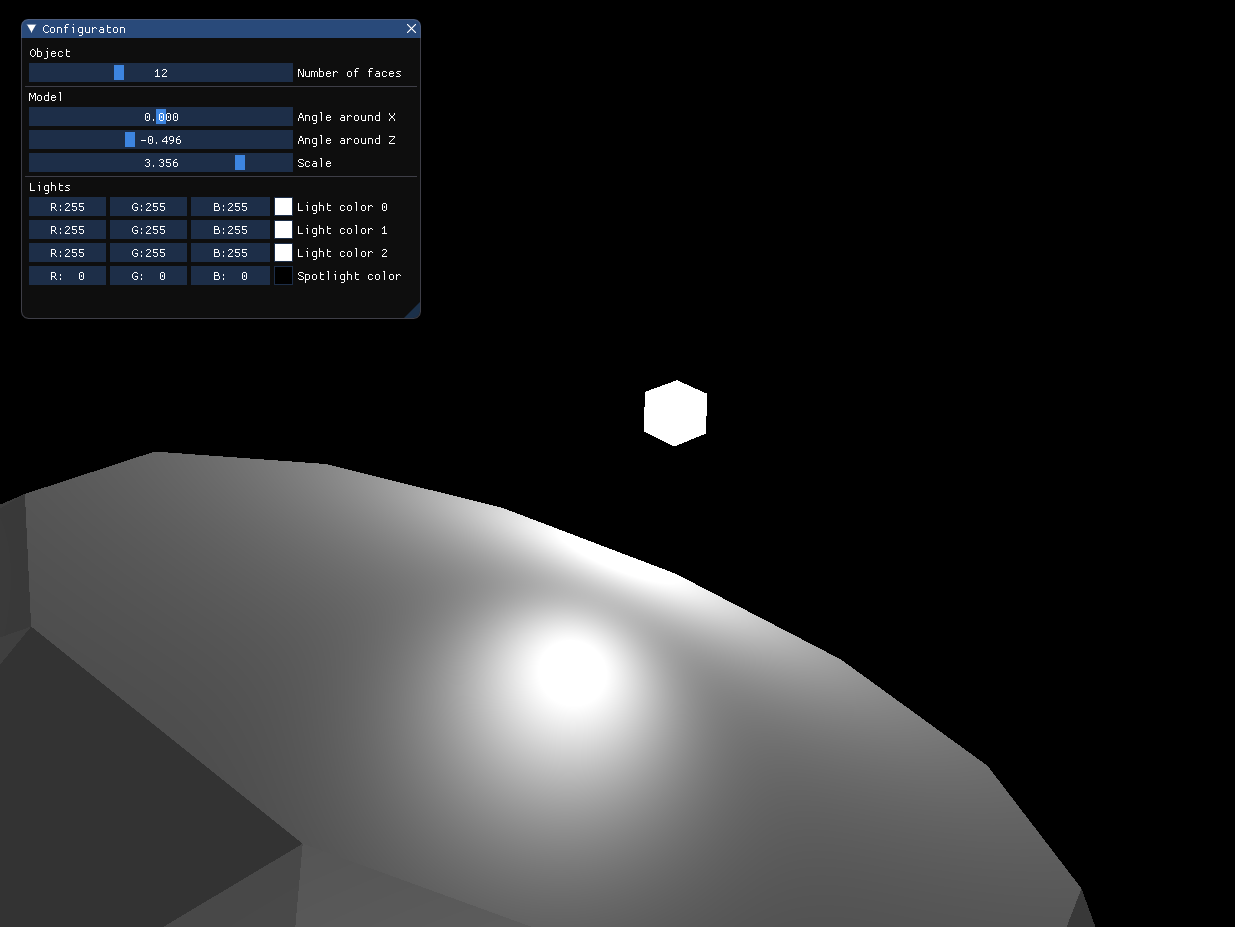
\includegraphics[width=0.9\textwidth]{screenshot_software_3}}

Notre implémentation nous permet de gérer un nombre arbitraire de lampes, le chiffre exact étant défini par des constantes
se trouvant dans le \textit{fragment shader} (configuré de manière arbitraire sur 5 lumières directionnelles, 15 lumières localisées et 15 spots au maximum).

